\documentclass[11pt,a4paper]{article}
\usepackage[utf8]{inputenc}
\usepackage[T1]{fontenc}
\usepackage[english]{babel}
\usepackage{lmodern}
\usepackage{microtype}
\usepackage{geometry}
\usepackage{graphicx}
\usepackage[table]{xcolor}
\usepackage{booktabs}
\usepackage{longtable}
\usepackage{tabularx}
\usepackage{multirow}
\usepackage{hyperref}
\usepackage{enumitem}
\usepackage{tikz}
\usepackage{fancyhdr}
\usepackage{titlesec}
\usepackage{caption}
\usepackage{setspace}
\usepackage{mdframed}
\usepackage{array}
\usepackage{amsmath}
\usepackage{makecell}
\usepackage{seqsplit}

\usetikzlibrary{arrows.meta,positioning,shapes.geometric}

% --- Brand palette ---
\definecolor{bfhblue}{HTML}{1a3a5c}
\definecolor{bfhaccent}{HTML}{2d6a8f}
\definecolor{tablehdr}{HTML}{e8eef4}
\definecolor{lightgray}{HTML}{f5f7fa}
\definecolor{stategreen}{HTML}{d4edda}
\definecolor{stateyellow}{HTML}{fff3cd}
\definecolor{statered}{HTML}{f8d7da}
\definecolor{stategreentext}{HTML}{155724}
\definecolor{stateyellowtext}{HTML}{856404}
\definecolor{stateredtext}{HTML}{721c24}
\definecolor{infobox}{HTML}{e8f4fd}
\definecolor{infoborder}{HTML}{2d6a8f}

\geometry{margin=2.4cm, top=2.6cm, bottom=2.8cm, headheight=22pt}
\setlength{\parindent}{0pt}
\usetikzlibrary{arrows.meta,positioning,shapes.geometric,shapes.multipart}
%\setlength{\parskip}{6pt}
\hypersetup{
    colorlinks=true,
    linkcolor=bfhblue,
    urlcolor=bfhaccent,
    citecolor=bfhblue,
    pdftitle={RTOS Project Work -- Electrical Outlet IoT},
    pdfauthor={Simone Pelascini, Aurelien Bollin}
}

\captionsetup{font=small, labelfont={bf,color=bfhblue}}

% Section titles
\titleformat{\section}
    {\Large\bfseries\color{bfhblue}}
    {\thesection}{0.75em}{}
    [\vspace{-0.3em}{\color{bfhaccent}\titlerule[0.6pt]}]
\titleformat{\subsection}
    {\large\bfseries\color{bfhblue!85!black}}
    {\thesubsection}{0.6em}{}
\titleformat{\subsubsection}
    {\normalsize\bfseries\color{bfhblue!70!black}}
    {\thesubsubsection}{0.5em}{}
\titlespacing*{\section}{0pt}{1.8ex plus .2ex}{1.1ex plus .1ex}
\titlespacing*{\subsection}{0pt}{1.3ex plus .1ex}{0.7ex plus .1ex}

\setlist{itemsep=0.3ex, topsep=0.6ex}

% Info box style
\mdfdefinestyle{infoboxstyle}{
    backgroundcolor=infobox,
    linecolor=infoborder,
    linewidth=1.2pt,
    leftline=true, rightline=false, topline=false, bottomline=false,
    innerleftmargin=10pt, innerrightmargin=8pt,
    innertopmargin=6pt, innerbottommargin=6pt,
    skipabove=6pt, skipbelow=6pt
}

% Header / footer
\pagestyle{fancy}
\fancyhf{}
\fancyhead[L]{\small\color{bfhblue}\textbf{Electrical Outlet IoT}}
\fancyhead[R]{\small\color{gray}\nouppercase{\leftmark}}
\fancyfoot[C]{%
\small
Bern University of Applied Sciences \textbar{}
Engineering and Computer Science \textbar{}
Electrical Engineering and Information Technology
}
\renewcommand{\headrulewidth}{0.4pt}
\renewcommand{\headrule}{\hbox to\headwidth{\color{bfhaccent}\leaders\hrule height \headrulewidth\hfill}}

\fancypagestyle{plain}{%
  \fancyhf{}
  \fancyfoot[C]{%
  \small
  Bern University of Applied Sciences \textbar{}
  Engineering and Computer Science \textbar{}
  Electrical Engineering and Information Technology
  }
  \renewcommand{\headrulewidth}{0pt}
}

% Helpers
\newcommand{\rowhdr}{\rowcolor{tablehdr}}
\newcommand{\stateImpl}{\cellcolor{stategreen}\textcolor{stategreentext}{\textbf{implemented}}}
\newcommand{\statePartial}{\cellcolor{stateyellow}\textcolor{stateyellowtext}{\textbf{partial}}}
\newcommand{\stateOpen}{\cellcolor{statered}\textcolor{stateredtext}{\textbf{open}}}

% ============================================================
\begin{document}

% ---------- Title page ----------
\begin{titlepage}
    \centering
    \vspace*{0.15cm}
    {\color{bfhblue}\rule{\textwidth}{2.2pt}}
    \vspace{0.55cm}

    {\Large\color{bfhaccent}Bern University of Applied Sciences\par}
    {\normalsize Engineering and Computer Science\par}
    {\normalsize Electrical Engineering and Information Technology\par}

    \vspace{1.2cm}
    {\Huge\bfseries\color{bfhblue}RTOS Project Work\par}
    \vspace{0.45cm}
    {\LARGE\color{bfhblue!80!black}Electrical Outlet IoT\par}
    \vspace{0.35cm}
    {\large Environmental monitoring node on ESP32 with FreeRTOS and MQTT\par}

    \vspace{1.6cm}
    \IfFileExists{../img/protoype.JPG}{%
        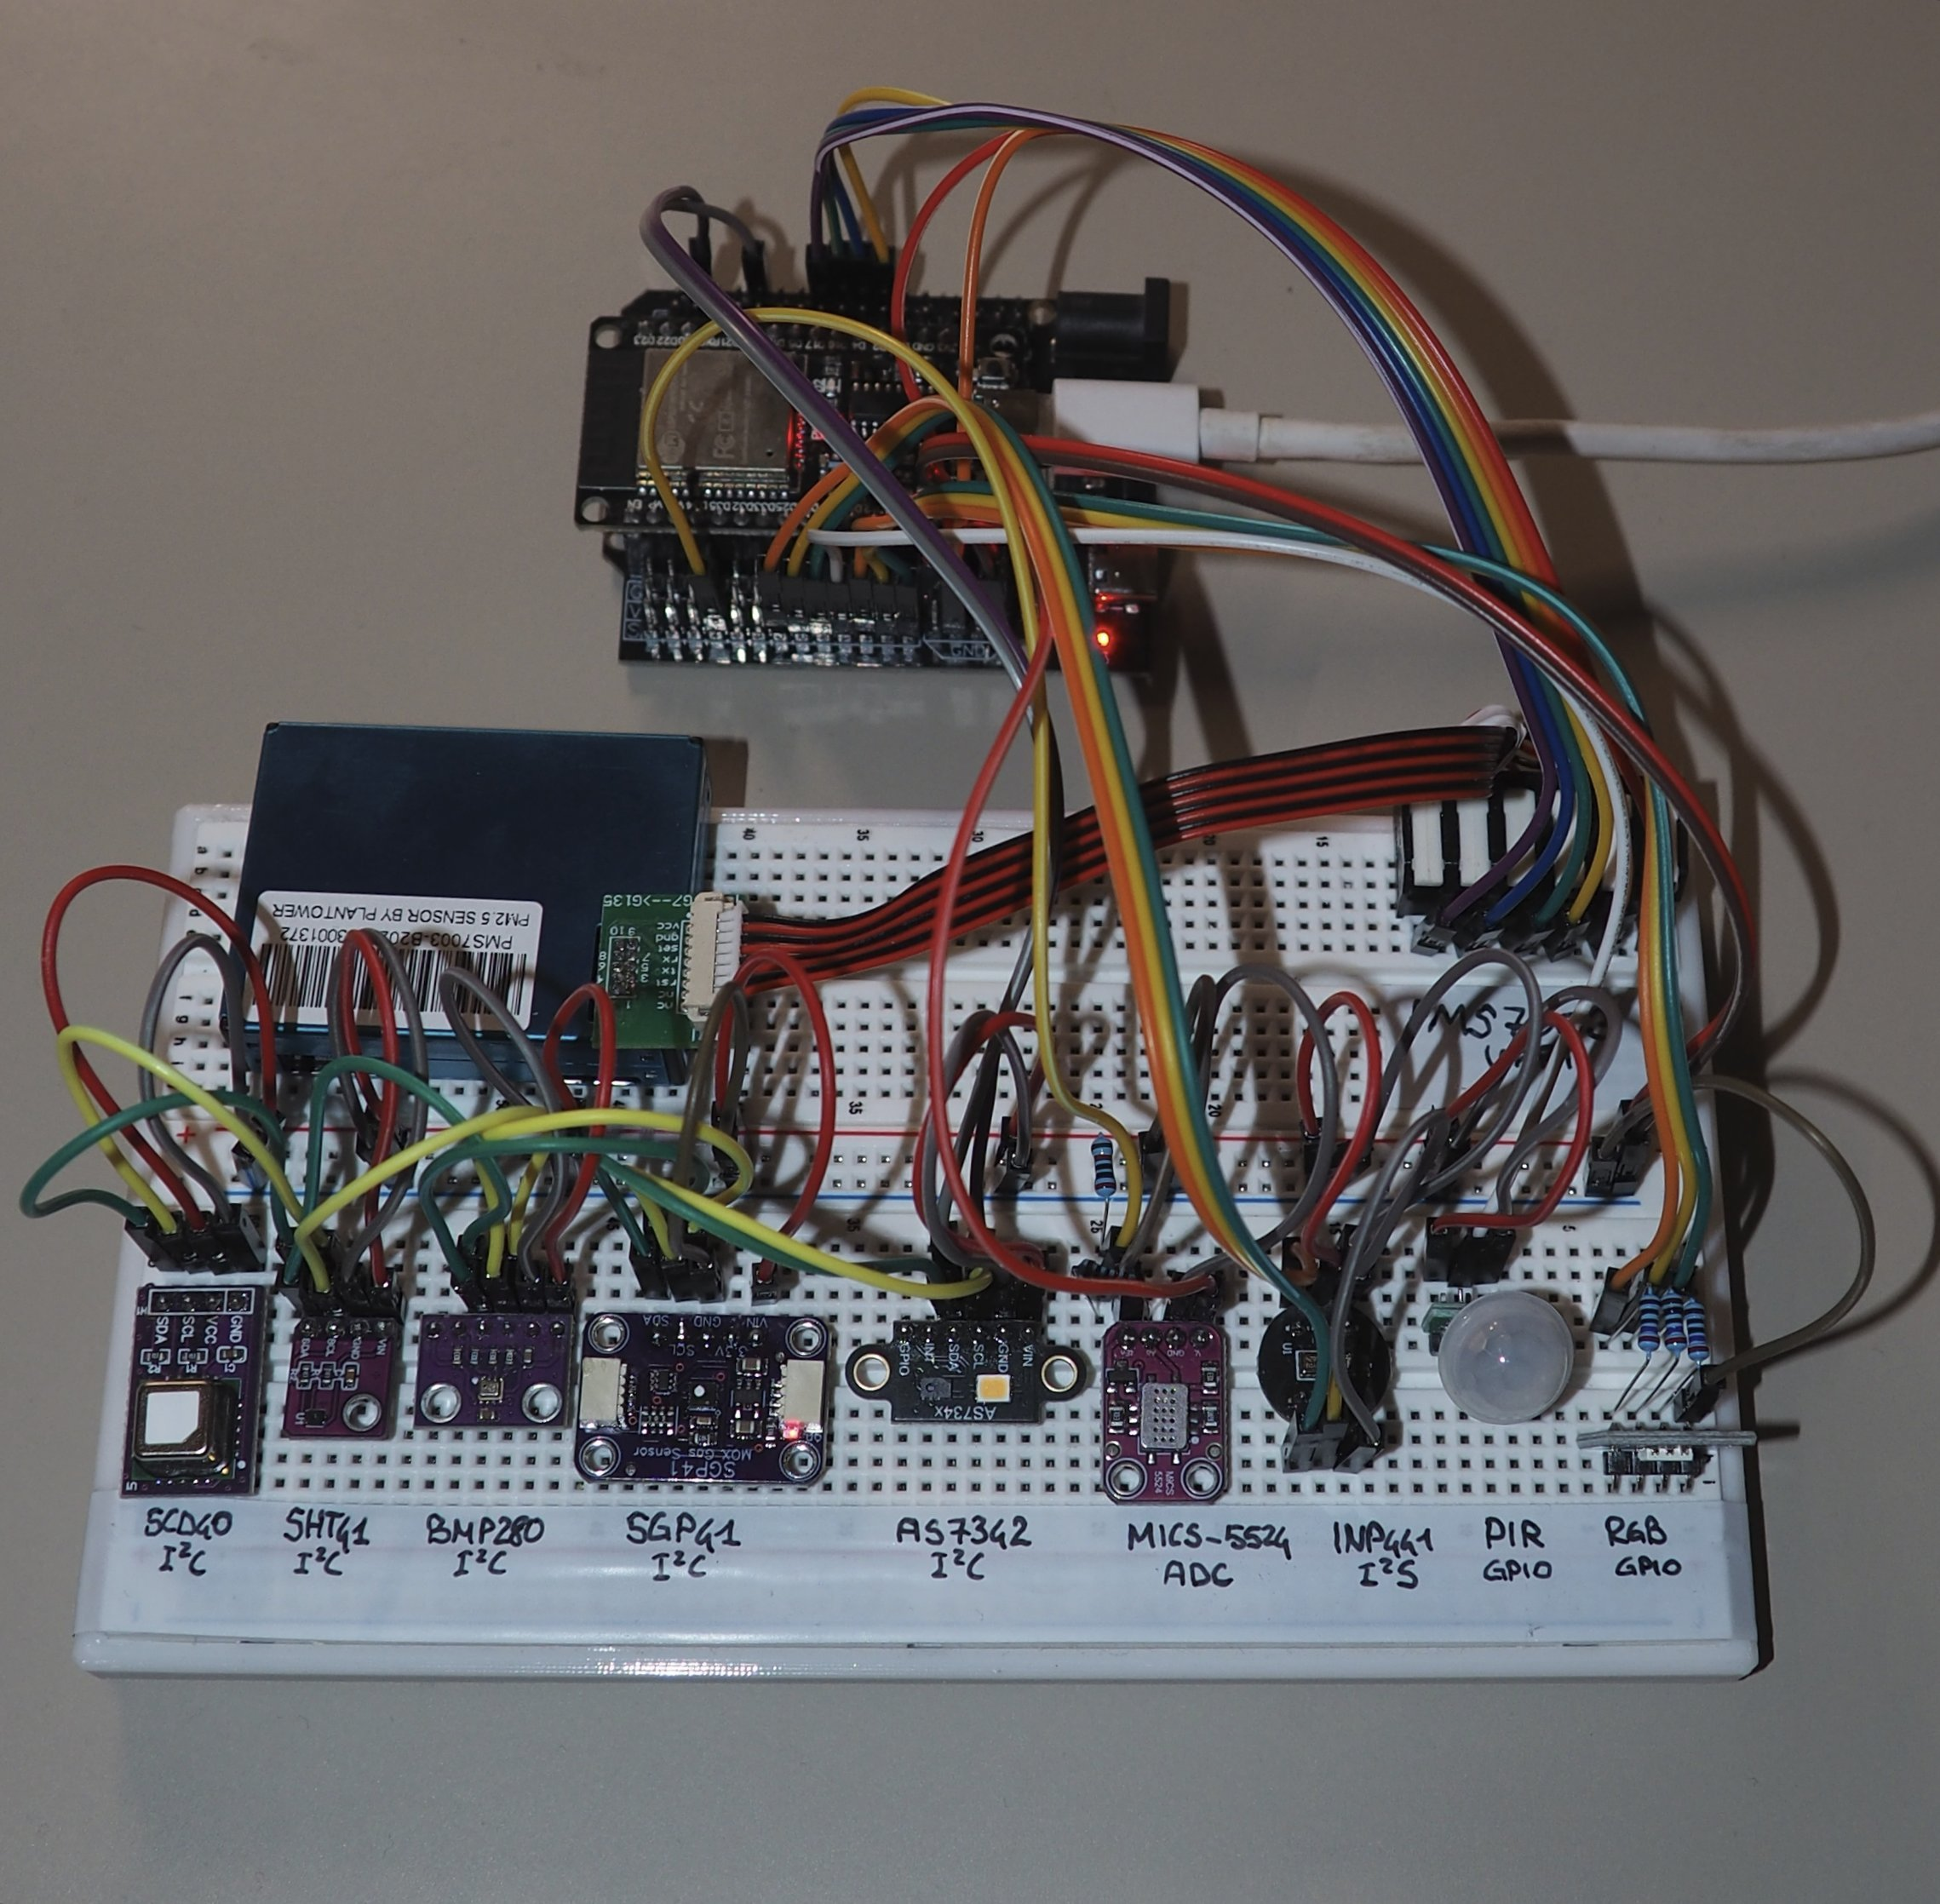
\includegraphics[width=0.60\textwidth]{../img/protoype.JPG}%
        \par\vspace{0.3em}
        {\small\color{gray}\textit{Breadboard prototype of the sensor node.}}
    }{%
        \fbox{\parbox{0.60\textwidth}{\centering\vspace{2.2cm}\texttt{../img/protoype.JPG} not found\vspace{2.2cm}}}%
    }

    \vfill
    {\large\textbf{Authors:} Simone Pelascini \quad\textbar\quad Aur\'elien Bollin\par}
    \vspace{0.6cm}
    {\large\textbf{Date:} \today\par}
    \vspace{1cm}
    {\color{bfhblue}\rule{\textwidth}{2pt}}
\end{titlepage}

\cleardoublepage
\pagenumbering{arabic}
\setcounter{page}{1}

\onehalfspacing
\tableofcontents
\newpage

% ============================================================
\section{Summary}
\vspace{10pt}

The \textbf{Electrical Outlet IoT} project is an ESP32-based environmental monitoring node designed to
be integrated into a standard wall-outlet form factor. The motivation behind this project is the growing
demand for \textbf{ambient air quality monitoring} and \textbf{occupancy-aware automation} in residential
and commercial buildings. Poor indoor air quality, driven by CO\textsubscript{2} accumulation,
volatile organic compounds (VOC), particulate matter (PM), and combustible gas, is a largely invisible
health risk. Existing commercial solutions are either too expensive, closed-source, or limited to a single
measurement type.

\vspace{5pt}

This project addresses that gap by combining nine sensors on a single node,
connected to a local MQTT broker for real-time telemetry. The firmware is built on \textit{PlatformIO},
\textit{ESP-IDF}, and \textit{FreeRTOS}, making use of four concurrent tasks that coordinate through
a \textbf{mutex-protected global state structure}. Sensor data is published as JSON payloads
and consumed by a companion Node.js dashboard that renders live charts via \textit{Chart.js}
and pushes updates to browsers via \textit{Socket.IO}.

\vspace{5pt}

The current repository documents breadboard bring-up, firmware architecture, runtime
characterisation, and the web-dashboard edge. The form-factor integration into an actual outlet housing
is left as a future step.

% ============================================================
\section{System Context}
\subsection{Hardware}
\vspace{5pt}

The sensor node is built around an \textbf{ESP32 dual-core 240~MHz} microcontroller (Espressif
\texttt{esp32dev} target). It communicates with nine sensors over five distinct interfaces.
Table~\ref{tab:sensors} summarises the complete sensor inventory.

{\footnotesize
\setlength{\tabcolsep}{4pt}
\renewcommand{\arraystretch}{1.1}

\rowcolors{2}{lightgray}{white}
\setlength\LTleft{0pt}
\begin{longtable}{@{}p{2.3cm}p{2.8cm}p{6cm}p{1.4cm}p{2.5cm}@{}}
\caption{Complete sensor inventory used by the ESP32 node.\label{tab:sensors}}\\
\rowhdr
\textbf{Sensor} & \textbf{Measured quantity} & \textbf{Physical value} & \textbf{Bus} & \textbf{Driver} \\
\midrule
\endhead
SCD40        & CO\textsubscript{2}, T, RH & Concentration, temperature, humidity & I\textsuperscript{2}C & Direct ESP-IDF \\
SHT41        & Temperature, humidity & High-precision T \& RH & I\textsuperscript{2}C & esp-idf-lib \\
SGP41        & VOC, NOx              & Gas indices 0--500 (Sensirion algorithm) & I\textsuperscript{2}C & Custom + GIA \\
BMP280       & Pressure, temperature & Atmospheric P \& T & I\textsuperscript{2}C & esp-idf-lib \\
AS7341       & Light spectrum        & 8-channel F1--F8 basic counts & I\textsuperscript{2}C & k0i05/esp\_as7341 \\
PMS7003      & Particulate matter    & PM1.0, PM2.5, PM10 [\textmu g/m\textsuperscript{3}] & UART & Custom wrapper \\
MiCS-5524    & Combustible gas       & Voltage [V], heuristic CO [ppm] & ADC & Custom \\
AS312        & PIR motion            & Motion detected (boolean) & GPIO & Custom \\
INMP441      & Ambient noise         & Sound pressure level [dB~SPL] & I\textsuperscript{2}S & Custom DSP \\
\bottomrule
\end{longtable}
\rowcolors{2}{}{}
}

\newpage

\subsection{System actors and data paths}
\vspace{5pt}

The system involves the following actors:
\begin{itemize}[leftmargin=*]
    \item \textbf{Sensor node}: ESP32 (\texttt{esp32dev}), firmware in \texttt{src/} and \texttt{lib/}.
          Samples all sensors on software-defined deadlines, aggregates readings into a shared
          in-memory state, and transmits them via Wi-Fi.
    \item \textbf{Wi-Fi / TCP}: the node connects as a Wi-Fi station; all MQTT traffic flows over
          a standard TCP connection to the broker.
    \item \textbf{MQTT broker}: any standard broker (e.g.\ Mosquitto) reachable on the LAN.
          Credentials and URI are configured in \texttt{lib/config/include/app\_config.h}.
    \item \textbf{Node.js dashboard}: an optional \texttt{server/} application that subscribes to
          all device topics and renders live charts in the browser via Socket.IO and Chart.js.
    \item \textbf{Third-party consumers}: any MQTT subscriber can access the JSON payloads
          independently of the dashboard.
\end{itemize}

\vspace{5pt}
\subsection{MQTT topics}
\vspace{5pt}

All publications follow the hierarchy \texttt{devices/\textless device\_id\textgreater /}
where \texttt{device\_id} is set by \texttt{\seqsplit{APP\_DEVICE\_ID}}:

\begin{itemize}[leftmargin=*]
    \item \texttt{telemetry/environment} (QoS~0) --- full sensor snapshot:
          CO\textsubscript{2}, T, RH from SCD40 and SHT41, atmospheric pressure, VOC/NOx indices,
          PM1.0/2.5/10, 8-channel light array, gas voltage and ppm, noise level in dB~SPL.
          Published every \textbf{1~s}.
    \item \texttt{\seqsplit{status/system}} (QoS~1, retain) --- system health flags:
          \texttt{\seqsplit{system\_ok}}, \texttt{\seqsplit{degraded\_mode}}, \texttt{\seqsplit{wifi\_connected}},
          \texttt{\seqsplit{mqtt\_connected}}. Published every \textbf{10~s} and immediately on reconnect.
    \item \texttt{\seqsplit{event/alarm}} (QoS~1) --- event-driven alert:
          \texttt{\seqsplit{as312\_alarm}} (motion), \texttt{\seqsplit{mics5524\_alarm}} (gas threshold exceeded),
          \texttt{\seqsplit{co2\_alarm\_level}} (IDA-inspired 6-level classification).
          Published only on the \textbf{rising edge} of each alarm flag.
\end{itemize}

\vspace{5pt}
\subsection{Web dashboard}
\vspace{5pt}

The companion dashboard runs on Node.js (\texttt{server/public/server.js}) and uses the
\texttt{\seqsplit{express}}, \texttt{\seqsplit{mqtt}}, \texttt{\seqsplit{socket.io}}, and \texttt{\seqsplit{dotenv}} packages. It subscribes
to the wildcard patterns \texttt{\seqsplit{devices/+/telemetry/environment}},
\texttt{\seqsplit{devices/+/status/system}}, and \texttt{\seqsplit{devices/+/event/alarm}}, merges incoming payloads
into a per-device state object, and forwards it to all connected browsers in real time.
Configuration is via a \texttt{.env} file (\texttt{\seqsplit{MQTT\_BROKER\_URL}}, optional credentials, \texttt{\seqsplit{PORT}}).

\newpage

% ============================================================
\section{Requirements}\label{sec:requirements}
\vspace{10pt}

Requirements are written from the user perspective and are traceable to implementation files.
The \textbf{State} column uses colour coding:
\colorbox{stategreen}{\textcolor{stategreentext}{implemented}},
\colorbox{stateyellow}{\textcolor{stateyellowtext}{partial}}, or
\colorbox{statered}{\textcolor{stateredtext}{open}}.

{\footnotesize
\setlength{\tabcolsep}{4pt}
\renewcommand{\arraystretch}{1.1}

\rowcolors{2}{lightgray}{white}
\setlength\LTleft{0pt}
\begin{longtable}{@{}>{\bfseries}p{0.9cm}p{11.6cm}p{3.0cm}@{}}
\caption{System requirements and current implementation status.\label{tab:requirements}}\\
\rowhdr
\multicolumn{1}{@{}l}{\textbf{ID}} & \textbf{Requirement (user perspective)} & \textbf{State} \\
\midrule
\endhead
R1 & The system shall boot, initialise all peripherals, create four FreeRTOS tasks, and reach a
     fully operational state without a fatal error within 20~s of power-on. & \stateImpl \\
R2 & The system shall connect to the configured Wi-Fi network within 15~s; on disconnect it shall
     retry up to \texttt{APP\_WIFI\_MAX\_RETRY} times automatically. & \stateImpl \\
R3 & The system shall publish a JSON environment payload to the MQTT broker at least every 1~s
     and a system-status payload every 10~s when connected. & \stateImpl \\
R4 & The system shall publish an alarm event payload on the rising edge of a motion or gas alarm,
     without missing edges caused by task jitter. & \stateImpl \\
R5 & All concurrent accesses to \texttt{g\_device\_state} shall be serialised by a FreeRTOS
     mutex (\texttt{g\_device\_state\_mutex}) with no unbounded blocking. & \stateImpl \\
R6 & All nine integrated sensors shall be polled within their specified deadlines without one
     slow sensor blocking another. & \stateImpl \\
R7 & The system shall report an estimated ambient noise level (\texttt{noise\_db}) in dB~SPL;
     absolute accuracy relative to a calibrated sound-level meter is not guaranteed without
     field calibration of \texttt{INMP441\_SPL\_OFFSET\_DB}. & \statePartial \\
R8 & Stack high-water mark and heap usage shall be logged and reported for all tasks over at
     least 10~minutes of continuous operation. & \stateImpl \\
R9 & Automated unit tests shall cover MQTT payload builders and sensor supervision logic. & \stateOpen \\
R10 & The system shall attempt automatic sensor restoration (re-initialisation and recovery) after
      a detected sensor crash, with bounded retries and fault reporting if recovery fails. & \stateOpen \\
\bottomrule
\end{longtable}
\rowcolors{2}{}{}
}

\newpage

% ============================================================
\section{Design}
\subsection{Boot sequence}
\vspace{5pt}

At startup, \texttt{app\_main} (in \texttt{src/main.c}) executes the following ordered steps.
All critical steps abort the system on failure; non-critical sensor failures are logged as
warnings and allow the system to continue in degraded mode.

\begin{enumerate}[leftmargin=*, label=\textbf{\arabic*.}]
    \item \textbf{\texttt{device\_state\_init()}} --- zero-initialises \texttt{g\_device\_state}
          and creates the two FreeRTOS mutexes (\texttt{g\_device\_state\_mutex} and
          \texttt{g\_sensor\_driver\_mutex}).
    \item \textbf{\texttt{sensor\_init\_all()}} --- initialises hardware peripherals in order:
          ADC unit~1, I\textsuperscript{2}S channel, I\textsuperscript{2}C bus, UART~2, then
          each sensor driver. Critical peripherals abort on failure; sensors warn and continue.
    \item \textbf{\texttt{network\_app\_init()}} --- initialises NVS, netif, Wi-Fi driver, and
          starts the connection; registers event handlers for \texttt{WIFI\_EVENT} and
          \texttt{IP\_EVENT}.
    \item \textbf{\texttt{\seqsplit{network\_app\_wait\_until\_connected(15000)}}} --- blocks up to 15~s
          waiting for \texttt{\seqsplit{APP\_WIFI\_CONNECTED\_BIT}}; aborts if the bit is not set.
    \item \textbf{\texttt{mqtt\_app\_start()}} --- creates the ESP-IDF MQTT client, registers
          the event handler, and starts the client task.
    \item \textbf{Task creation} --- \texttt{xTaskCreate} is called for each of the four tasks;
          any allocation failure aborts immediately.
\end{enumerate}

\newpage

\subsection{FreeRTOS task architecture}

The firmware is decomposed into four independent FreeRTOS tasks. All tasks use
\texttt{vTaskDelayUntil} for deterministic loop periods and \texttt{xSemaphoreTake} /
\texttt{xSemaphoreGive} for exclusive access to the shared state. Table~\ref{tab:tasks} summarises
the static parameters.

{\footnotesize
\setlength{\tabcolsep}{4pt}
\renewcommand{\arraystretch}{1.1}

\rowcolors{2}{lightgray}{white}
\setlength\LTleft{0pt}
\begin{longtable}{@{}p{3.1cm}p{7.6cm}ccp{2.0cm}@{}}
\caption{Static configuration of the four FreeRTOS tasks.\label{tab:tasks}}\\
\rowhdr
\textbf{Task} & \textbf{Responsibility} & \textbf{Pri.} & \textbf{Stack (w)} & \textbf{Period} \\
\midrule
\endhead
\texttt{acquisition\_task} & Polls all sensors on individual software deadlines; writes measured
  values, validity flags, and fault flags into \texttt{g\_device\_state} under the mutex. & 2 & 4096 & 1000~ms \\
\texttt{audio\_task} & DMA-reads one audio block from the INMP441 via I\textsuperscript{2}S,
  computes AC-RMS SPL, and updates \texttt{noise\_db} in the shared state. & 2 & 4096 & 500~ms \\
\texttt{comm\_task} & Snapshots the shared state and drives the MQTT publish schedule:
  environment telemetry at 1~s, system status at 10~s, and alarm events on rising edge. & 3 & 4096 & 100~ms \\
\texttt{system\_task} & Reads the shared state snapshot, evaluates per-sensor health checks
  (staleness, fault, validity) and alarm logic, then writes derived system flags back. & 4 & 4096 & 100~ms \\
\bottomrule
\end{longtable}
\rowcolors{2}{}{}
}

\vspace{5pt}
\begin{mdframed}[style=infoboxstyle]
\textbf{Design pattern --- local state before commit.}
Each task maintains a task-local state structure initialised to zero. Sensor readings and flags are
written to this local copy first; only when a consistent update is ready is the mutex acquired and
the global \texttt{g\_device\_state} updated in a single block-copy. This minimises the critical
section duration and avoids partially-updated state being observed by other tasks.
\end{mdframed}

\subsection{Sensor polling intervals}

Sensors inside \texttt{\seqsplit{acquisition\_task}} are polled on independent software timers derived from
\texttt{\seqsplit{xTaskGetTickCount()}}. Each sensor deadline is checked at every 1000~ms task tick; the
sensor is read only when \texttt{now - last\_read \(\geq\) interval}. This means a single slow
sensor (e.g.\ PMS7003) does not delay faster ones (e.g.\ AS312).

\vspace{8pt}

{\footnotesize
\setlength{\tabcolsep}{4pt}
\renewcommand{\arraystretch}{1.1}

\noindent
\captionof{table}{Sensor polling intervals and interfaces used by the firmware.\label{tab:polling_intervals}}
\begin{tabularx}{\textwidth}{@{}lXrr@{}}
\toprule
\rowhdr
\textbf{Sensor} & \textbf{Physical quantity} & \textbf{Interface} & \textbf{Interval} \\
\midrule
AS312  & PIR motion                         & GPIO                          & 1000~ms \\
MiCS-5524 & Combustible gas (CO heuristic)  & ADC                           & 1000~ms \\
SGP41  & VOC index, NOx index               & I\textsuperscript{2}C         & 1000~ms \\
AS7341 & 8-channel light spectrum           & I\textsuperscript{2}C         & 1000~ms \\
SHT41  & Temperature, humidity              & I\textsuperscript{2}C         & 2000~ms \\
BMP280 & Atmospheric pressure               & I\textsuperscript{2}C         & 2000~ms \\
SCD40  & CO\textsubscript{2}, temperature, humidity & I\textsuperscript{2}C  & 2500~ms \\
PMS7003 & PM1.0, PM2.5, PM10               & UART                          & 5000~ms \\
INMP441 & Noise level (dB SPL)             & I\textsuperscript{2}S (audio\_task) & 500~ms \\
\bottomrule
\end{tabularx}
}

\newpage

\subsection{System supervision and alarm logic}

\texttt{system\_task} implements two independent modules:

\textbf{Health module} (\texttt{lib/health/}): after a 45~s cold-start window, each sensor
is checked for three conditions: (1) the validity flag is \texttt{false}, (2) the fault flag is
\texttt{true}, or (3) the timestamp age exceeds a per-sensor timeout (45~s for all sensors).
Any failing check sets \texttt{degraded\_mode = true} and the sensor-specific \texttt{degraded\_*}
flag.

\textbf{Alarm module} (\texttt{lib/alarm/}): three independent sub-checks evaluate
(1)~motion from the AS312 PIR, (2)~gas concentration from MiCS-5524 against a 5000~ppm threshold,
and (3)~CO\textsubscript{2} from SCD40 classified into six levels (Optimal / Good / Moderate /
Poor / Very Poor / Critical) following IDA and ASHRAE~62.1-inspired thresholds.

\subsection{System context diagram}
\vspace{5pt}

\begin{figure}[!htbp]
\centering
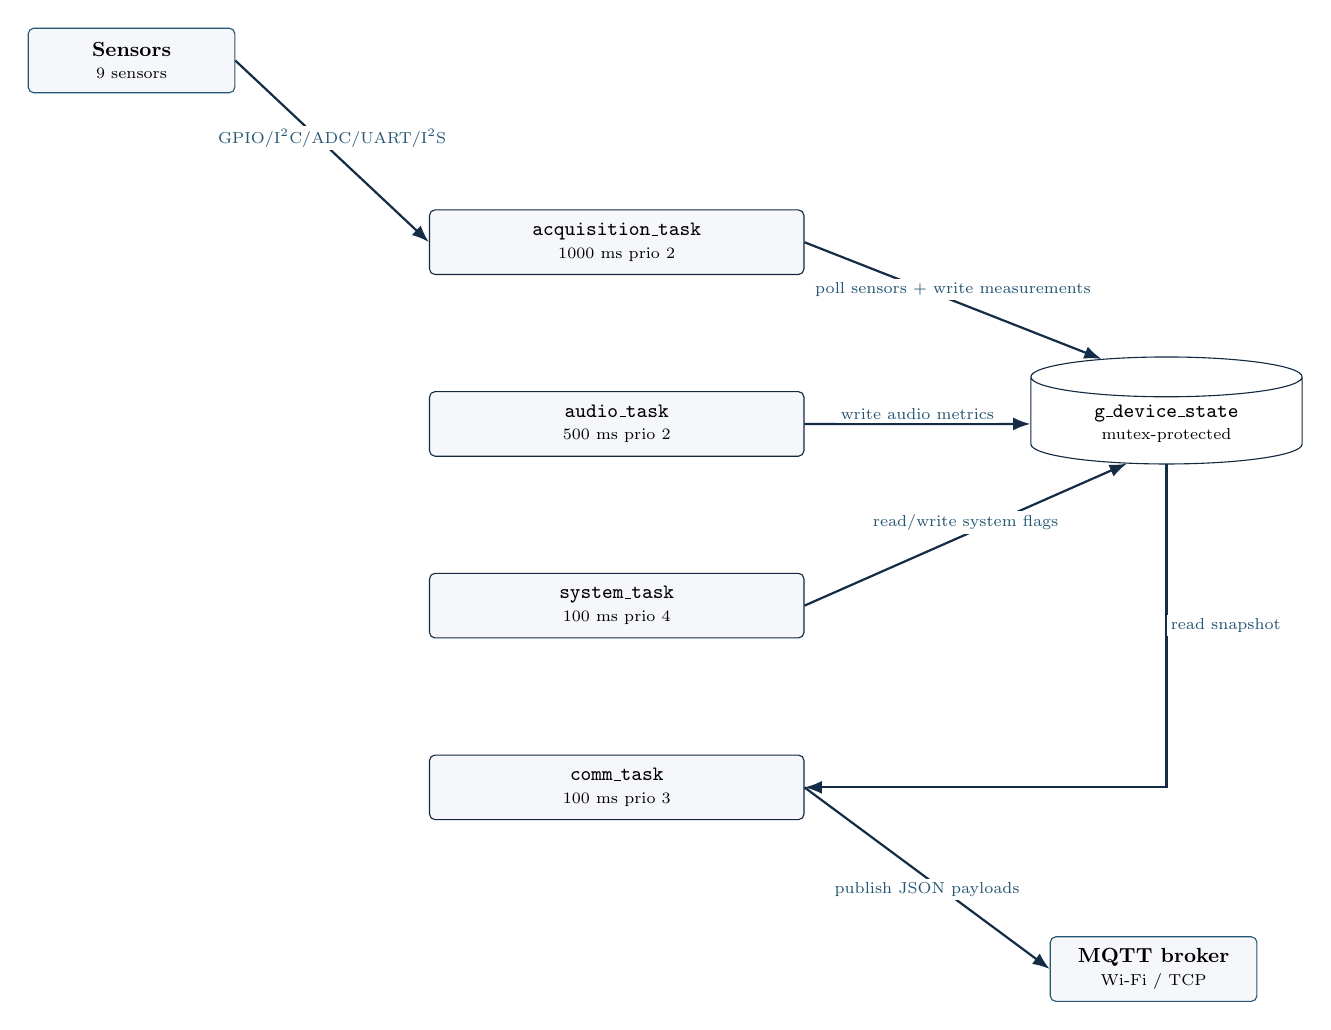
\begin{tikzpicture}[
    scale=0.82,
    transform shape,
    node distance=9mm and 18mm,
    task/.style={
        draw=bfhblue!70!black,
        rounded corners=2pt,
        align=center,
        minimum width=58mm,
        minimum height=10mm,
        fill=lightgray,
        font=\small
    },
    state/.style={
        draw=bfhblue!70!black,
        cylinder,
        shape border rotate=90,
        aspect=0.25,
        align=center,
        minimum width=42mm,
        minimum height=13mm,
        fill=white,
        font=\small
    },
    ext/.style={
        draw=bfhaccent!80!black,
        rounded corners=2pt,
        align=center,
        minimum width=32mm,
        minimum height=10mm,
        fill=lightgray,
        font=\small
    },
    arrow/.style={
        -{Latex[length=2.2mm]},
        thick,
        color=bfhblue!75!black
    },
    label/.style={
        font=\scriptsize,
        fill=white,
        inner sep=1.5pt,
        text=bfhaccent!80!black
    }
]

% Sensors block
\node[ext] (sensors)
{\textbf{Sensors}\\[-1pt]\scriptsize 9 sensors};

% Tasks
\node[task, below right=18mm and 30mm of sensors] (acq)
{\texttt{acquisition\_task}\\[-1pt]\scriptsize 1000~ms prio 2};

\node[task, below=18mm of acq] (audio)
{\texttt{audio\_task}\\[-1pt]\scriptsize 500~ms prio 2};

\node[task, below=18mm of audio] (system)
{\texttt{system\_task}\\[-1pt]\scriptsize 100~ms prio 4};

\node[task, below=18mm of system] (comm)
{\texttt{comm\_task}\\[-1pt]\scriptsize 100~ms prio 3};

% Shared state and MQTT
\node[state, right=35mm of audio] (devstate)
{\texttt{g\_device\_state}\\[-1pt]\scriptsize mutex-protected};

\node[ext, below right=18mm and 38mm of comm] (mqtt)
{\textbf{MQTT broker}\\[-1pt]\scriptsize Wi-Fi / TCP};

% Connections
\draw[arrow] (sensors.east) -- node[label, above]
{GPIO/I\textsuperscript{2}C/ADC/UART/I\textsuperscript{2}S}
(acq.west);

\draw[arrow] (acq.east) -- node[label, above]
{poll sensors + write measurements}
(devstate.north west);

\draw[arrow] (audio.east) -- node[label, above]
{write audio metrics}
(devstate.west);

\draw[arrow] (system.east) -- node[label, above]
{read/write system flags}
(devstate.south west);

\draw[arrow] (devstate.south) |- node[label, near start, right]
{read snapshot}
(comm.east);

\draw[arrow] (comm.east) -- node[label, below]
{publish JSON payloads}
(mqtt.west);

\end{tikzpicture}

\caption{System context diagram showing sensors, FreeRTOS tasks, the mutex-protected shared state,
and the MQTT broker used for publishing telemetry, status, and alarm messages.}
\end{figure}

\newpage

\subsection{UML task interaction diagram}

\begin{figure}[!htbp]
\centering
\IfFileExists{../img/uml_4task.png}{%
    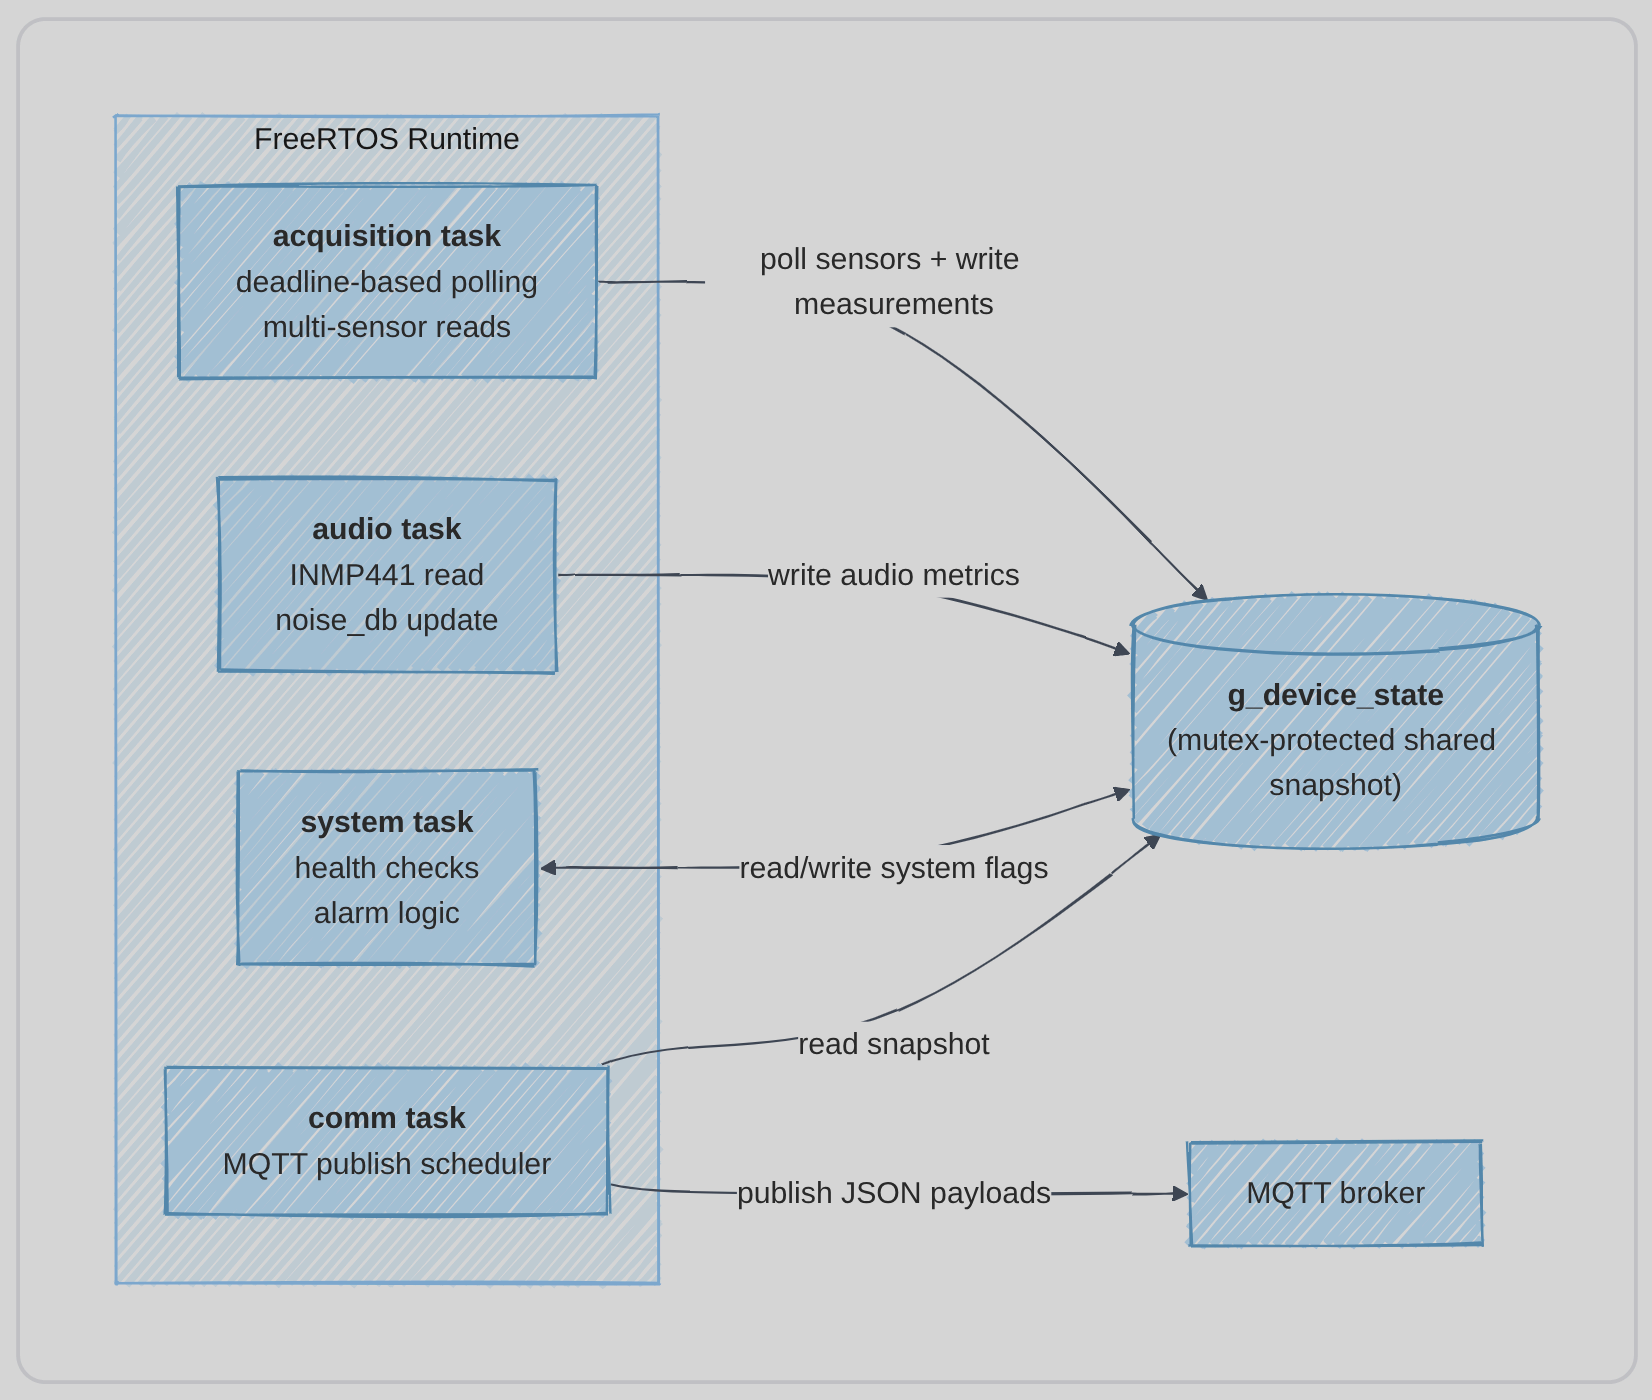
\includegraphics[width=0.88\textwidth]{../img/uml_4task.png}%
}{%
    \fbox{\parbox{0.88\textwidth}{\centering\vspace{1.8cm}
    \texttt{../img/uml\_4task.png} not found\vspace{1.8cm}}}%
}
\caption{UML activity/sequence diagram of the four FreeRTOS tasks and their interactions
with \texttt{g\_device\_state} and the MQTT client.}
\end{figure}

\subsection{Acquisition polling flow}

\begin{figure}[!htbp]
\centering
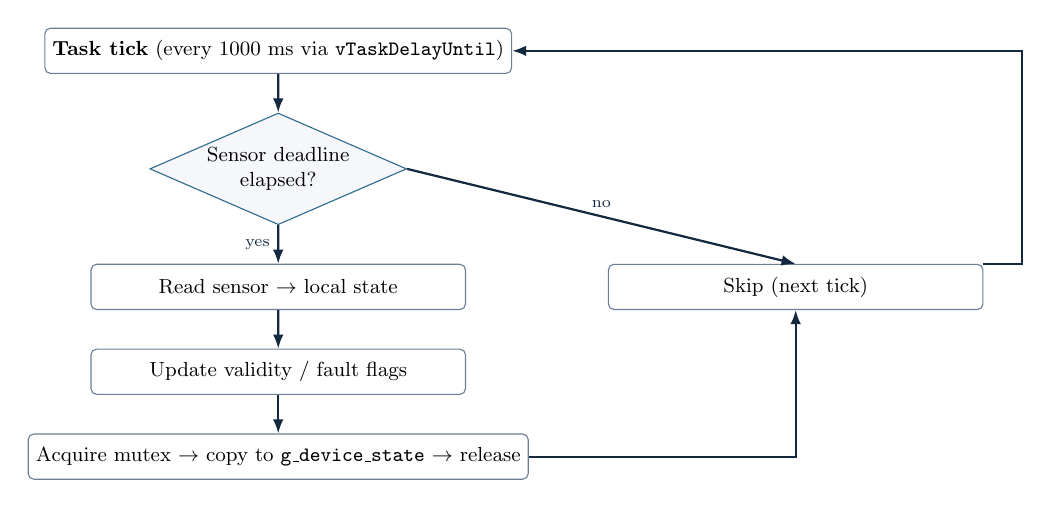
\begin{tikzpicture}[
    scale=0.82,
    transform shape,
    node distance=6mm,
    proc/.style={draw=bfhblue!65, rounded corners=2pt, align=center,
                 minimum width=58mm, minimum height=7mm, fill=white, font=\small},
    dec/.style={draw=bfhaccent, diamond, aspect=2.3, align=center,
                inner sep=1pt, fill=lightgray, font=\small},
    arrow/.style={-{Latex[length=1.8mm]}, thick, color=bfhblue!70!black}
]
\node[proc] (loop) {\textbf{Task tick} (every 1000~ms via \texttt{vTaskDelayUntil})};
\node[dec, below=of loop] (due) {Sensor deadline\\ elapsed?};
\node[proc, below=of due] (read) {Read sensor $\rightarrow$ local state};
\node[proc, below=of read] (flag) {Update validity / fault flags};
\node[proc, below=of flag] (commit) {Acquire mutex $\rightarrow$ copy to \texttt{g\_device\_state} $\rightarrow$ release};
\node[proc, right=22mm of read] (skip) {Skip (next tick)};

\draw[arrow] (loop) -- (due);
\draw[arrow] (due) -- node[left, font=\scriptsize] {yes} (read);
\draw[arrow] (read) -- (flag);
\draw[arrow] (flag) -- (commit);
\draw[arrow] (commit.east) -| (skip.south);
\draw[arrow] (due.east) -- node[above, font=\scriptsize] {no} (skip.north);
\draw[arrow] (skip.north east) -- ++(6mm,0) |- (loop.east);
\end{tikzpicture}
\caption{Deadline-driven polling inside \texttt{acquisition\_task}: each sensor has its own
independent timer; skipped sensors do not block the loop.}
\end{figure}

\newpage

% ============================================================
\section{Runtime Statistics}\label{sec:runtime}

\subsection{Methodology}
\vspace{5pt}

Runtime measurements were collected from the ESP32 serial log using the helper functions
\texttt{logTaskStackHeapUsage()} and \texttt{logTaskAlive()}, defined in
\texttt{src/task\_config.c}. Each task logs its own stack high-water mark and the system-wide
heap state every \textbf{10~s} of wall-clock time. The measurements span approximately
\textbf{10~minutes} of continuous operation under normal conditions (all sensors active,
Wi-Fi connected, MQTT publishing running). Raw data is archived in
\texttt{raport/project\_info/stack\_heap.txt}.

Stack usage percentage is computed as:
\[
\text{Stack Usage} = \frac{\text{words used (high-water mark)}}{\text{stack allocated (words)}} \times 100\%
\]
where \emph{words used} = allocated $-$ high-water mark remaining (reported by
\texttt{\seqsplit{uxTaskGetStackHighWaterMark()}}; 1~word~= 4~bytes on ESP32).

\subsection{Stack usage per task}

\vspace{5pt}
{\footnotesize
\setlength{\tabcolsep}{4pt}
\renewcommand{\arraystretch}{1.1}

\rowcolors{2}{lightgray}{white}
\setlength\LTleft{0pt}
\begin{longtable}{@{}p{3.0cm}p{1.5cm}p{2.5cm}p{2.5cm}p{2.5cm}p{2.5cm}@{}}
\caption{Measured stack usage per FreeRTOS task over the runtime window.\label{tab:stack_usage}}\\
\rowhdr
\textbf{Task} & \textbf{Pri.} &
\makecell[c]{\textbf{Stack}\\\textbf{alloc. (w)}} &
\makecell[c]{\textbf{Stack used}\\\textbf{(HWM, w)}} &
\makecell[c]{\textbf{Usage}\\\textbf{(\%)}} &
\makecell[c]{\textbf{Avg. CPU}\\\textbf{(\%)}} \\
\midrule
\endhead
\texttt{acquisition\_task} & 2 & 4096 & 2532 & 61.8\% & n/m \\
\texttt{audio\_task}       & 2 & 4096 & 2124 & 51.9\% & n/m \\
\texttt{comm\_task}        & 3 & 4096 & 2812 & 68.7\% & n/m \\
\texttt{system\_task}      & 4 & 4096 & 2352 & 57.4\% & n/m \\
\bottomrule
\end{longtable}
\rowcolors{2}{}{}
}
{\small\textit{n/m = not measured (FreeRTOS runtime stats counter not enabled in this build).}}

\medskip
\begin{mdframed}[style=infoboxstyle]
\textbf{Stack analysis.}
The highest consumer is \texttt{comm\_task} (68.7\%), followed by \texttt{acquisition\_task}
(61.8\%). Even the worst case leaves \textbf{1284~words (5136~bytes) of free stack headroom}
on \texttt{comm\_task}, well above the ESP-IDF recommended minimum of 512~bytes. No stack
overflow was observed during the measurement window. All four stacks are sized safely at the
current feature set; if JSON payload building or additional sensors are added,
\texttt{comm\_task} should be monitored first.
\end{mdframed}

\newpage

\subsection{Heap usage over time}

The heap figures below are system-wide (MALLOC\_CAP\_8BIT pool, total $\approx$~290~KB).
``Min free'' is the all-time minimum free heap reported by
\texttt{heap\_caps\_get\_minimum\_free\_size}, which is the most conservative safety margin.

\vspace{5pt}
{\footnotesize
\setlength{\tabcolsep}{4pt}
\renewcommand{\arraystretch}{1.1}

\rowcolors{2}{lightgray}{white}
\setlength\LTleft{0pt}
\begin{longtable}{@{}p{2.6cm}p{2.3cm}p{2.3cm}p{2.5cm}p{1.5cm}p{3.5cm}@{}}
\caption{System heap usage at three measurement windows.\label{tab:heap}}\\
\rowhdr
\textbf{Window} &
\textbf{Used (B)} &
\textbf{Free (B)} &
\textbf{Min free (B)} &
\textbf{Usage} &
\textbf{Notes} \\
\midrule
\endhead
$\sim$10~s  & 107\,460 & 183\,116 & 176\,968 & 37.0\% & Post-boot steady state \\
$\sim$1~min & 107\,452 & 183\,124 & 176\,968 & 37.0\% & Stable; marginal drift \\
$\sim$10~min & 107\,432 & 183\,144 & 176\,968 & 37.0\% & Stable baseline \\
Peak (transient) & 108\,992 & 181\,584 & 176\,968 & 37.5\% & Acquisition spike \\
\bottomrule
\end{longtable}
\rowcolors{2}{}{}

}

\vspace{5pt}
\begin{mdframed}[style=infoboxstyle]
\textbf{Heap analysis.}
Heap usage is highly stable at approximately \textbf{37\%} of the total $\approx$290~KB pool,
leaving a comfortable \textbf{63\% free} ($\approx$183~KB) during steady-state operation.
The minimum-free-ever figure of \textbf{176\,968~B} ($\approx$173~KB) confirms that even
transient allocation peaks (up to 108\,992~B used, observed periodically during
\texttt{acquisition\_task} sensor reads) do not threaten memory safety.
Importantly, the baseline heap usage \emph{decreased} slightly over 10~minutes (from 107\,460~B
to 107\,432~B), indicating that there are \textbf{no measurable memory leaks} over the
observation window.
\end{mdframed}

\newpage

% ============================================================
\section{File Structure}
\vspace{10pt}

The repository follows the PlatformIO convention with a \texttt{src/} entry point, a
\texttt{lib/} folder for reusable modules, and a top-level \texttt{include/} for headers
shared across tasks. Each library module lives in its own subdirectory with an \texttt{include/}
header folder and a \texttt{src/} implementation folder, making cross-compilation units and
Doxygen generation straightforward.

\vspace{5pt}
{\footnotesize
\setlength{\tabcolsep}{4pt}
\renewcommand{\arraystretch}{1.1}

\rowcolors{2}{lightgray}{white}
\begin{longtable}{@{}p{3.5cm}p{12.2cm}@{}}
\caption{Repository file structure and module responsibilities.\label{tab:file_structure}}\\
\rowhdr
\textbf{Path} & \textbf{Purpose} \\
\midrule
\endhead
\texttt{src/} & Application entry point (\texttt{main.c}) and the four FreeRTOS task implementations:
  \texttt{acquisition\_task.c}, \texttt{audio\_task.c}, \texttt{comm\_task.c},
  \texttt{system\_task.c}. Also contains \texttt{task\_config.c} (stack/heap logging helpers)
  and \texttt{idf\_component.yml} (managed component manifest). \\
\texttt{include/} & Shared task headers (\texttt{*\_task.h}); \texttt{task\_config.h} defining
  stack sizes, task priorities, sensor polling intervals, and MQTT publish cadences. \\
\texttt{lib/config/} & \texttt{app\_config\_template.h} (Wi-Fi, MQTT, QoS, device ID constants)
  and \texttt{esp32\_pinout.h} (GPIO/peripheral pin assignments). \\
\texttt{lib/device\_state/} & Global \texttt{g\_device\_state} struct and the two FreeRTOS
  mutexes; all sensor values, timestamps, validity/fault flags, and system flags. \\
\texttt{lib/network/} & Wi-Fi station init (\texttt{network\_app.c}): NVS, netif, event handlers,
  reconnect logic, and the connection-ready event group. \\
\texttt{lib/mqtt/} & Four modules: \texttt{mqtt\_app} (client lifecycle), \texttt{mqtt\_topic}
  (topic string builders), \texttt{mqtt\_payload} (JSON serialisers),
  \texttt{mqtt\_publish} (high-level publish API). \\
\texttt{lib/sensor\_init/} & Peripheral bring-up: \texttt{adc\_init}, \texttt{i2s\_init},
  \texttt{uart\_init} (individual units), and \texttt{sensor\_init} (orchestrates all). \\
\texttt{lib/} (drivers) & One folder per sensor: \texttt{scd40}, \texttt{sht41}, \texttt{sgp41},
  \texttt{bmp280}, \texttt{as7341}, \texttt{pms7003}, \texttt{mics5524}, \texttt{as312},
  \texttt{inmp441}. Plus \texttt{health} (supervision), \texttt{alarm} (event logic),
  \texttt{rgbled} (status LED). \\
\texttt{lib/sgp41/include/} & Also contains Sensirion's BSD-3 Gas Index Algorithm header
  (\texttt{sensirion\_gas\_index\_algorithm.h}). \\
\texttt{server/} & Node.js dashboard: \texttt{public/server.js} (MQTT subscriber +
  Socket.IO relay), \texttt{app.js}, \texttt{index.html}, \texttt{style.css},
  \texttt{package.json}. \\
\texttt{scripts/} & \texttt{update\_clangd\_toolchain.py}: PlatformIO post-build hook that
  patches \texttt{.clangd} with the correct ESP-IDF include paths for IDE support. \\
\texttt{platformio.ini} & Build configuration: \texttt{esp32dev} target, ESP-IDF framework,
  4~MB flash, 115200~baud monitor, post-build extra script. \\
\texttt{raport/} & This report (\texttt{raport.tex}), the BFH template PDF,
  and \texttt{project\_info/} with raw measurement logs. \\
\bottomrule
\end{longtable}
\rowcolors{2}{}{}

}

\newpage
% ============================================================
\section{User Manual}
\vspace{10pt}

\begin{mdframed}[style=infoboxstyle]
\textbf{Prerequisite:} the ESP32 has already been flashed with the firmware.
You need a Wi-Fi network and an MQTT broker (e.g.\ Mosquitto) reachable on the same LAN.
\end{mdframed}

\subsection{Step 1 --- Configure credentials}

Open \texttt{lib/config/include/app\_config.h} and fill in your values:

\begin{verbatim}
#define APP_WIFI_SSID        "YourNetworkSSID"
#define APP_WIFI_PASSWORD    "YourNetworkPassword"
#define APP_MQTT_BROKER_URI  "mqtt://192.168.1.10"   // broker IP
#define APP_DEVICE_ID        "esp32_node_01"         // unique ID
\end{verbatim}

Leave \texttt{APP\_MQTT\_USERNAME} and \texttt{APP\_MQTT\_PASSWORD} empty if your broker has no
authentication. Rebuild and re-flash after editing this file.

\subsection{Step 2 --- Flash and monitor}

From the repository root, run:

\begin{verbatim}
# Build, upload, and open serial monitor (115200 baud)
pio run -t upload && pio device monitor -b 115200
\end{verbatim}

If the serial port is not detected automatically, add \texttt{upload\_port = /dev/ttyUSB0}
(or the appropriate port) to \texttt{platformio.ini}.

\subsection{Step 3 --- Verify boot sequence}

Watch the serial output. A successful startup prints, in order:

\begin{enumerate}[leftmargin=*, label=\textbf{\arabic*.}]
    \item \texttt{[MAIN] System booting...}
    \item \texttt{[MAIN] Sensors initialized successfully}
    \item \texttt{[MAIN] Wi-Fi connected successfully}
    \item \texttt{[MAIN] Starting MQTT}
    \item \texttt{MQTT\_APP: MQTT client started}
    \item \texttt{[MAIN] All tasks started}
\end{enumerate}

If any step fails, the system prints an error and calls \texttt{abort()}. Check credentials
(\texttt{app\_config.h}), broker reachability (ping from the same subnet), and GPIO wiring.

\newpage
\subsection{Step 4 --- Subscribe to MQTT topics}

Use any MQTT client to verify the data stream. Example with \texttt{mosquitto\_sub}:

\begin{verbatim}
# All topics for this device
mosquitto_sub -h 192.168.1.10 -t "devices/esp32_node_01/#" -v

# Environment telemetry only
mosquitto_sub -h 192.168.1.10 \
  -t "devices/esp32_node_01/telemetry/environment" -v
\end{verbatim}

You should see a new JSON payload roughly every second on the environment topic.

\subsection{Step 5 --- Start the web dashboard (optional)}

\begin{verbatim}
cd server
npm install                    # first run only
cp .env.example .env           # create local config
\end{verbatim}

Edit \texttt{.env} and set \texttt{MQTT\_BROKER\_URL=mqtt://192.168.1.10} (and
\texttt{PORT} if needed), then:

\begin{verbatim}
npm start
\end{verbatim}

Open \texttt{http://localhost:3000} (or the configured port) in a browser. Live charts for all
sensor channels update automatically via Socket.IO.

\subsection{Troubleshooting}

\begin{itemize}[leftmargin=*]
    \item \textbf{Wi-Fi fails}: verify SSID/password in \texttt{app\_config.h}; check that the
          access point uses WPA2-PSK.
    \item \textbf{MQTT fails}: ping the broker from the LAN; ensure \texttt{APP\_MQTT\_BROKER\_URI}
          starts with \texttt{mqtt://} and uses the correct IP and port (default 1883).
    \item \textbf{Sensor missing from payload}: check wiring against \texttt{esp32\_pinout.h};
          the \texttt{degraded\_mode} flag in \texttt{status/system} will be \texttt{true}
          after 45~s if a sensor stops responding.
    \item \textbf{Noise level seems wrong}: the \texttt{INMP441\_SPL\_OFFSET\_DB} constant in
          \texttt{\seqsplit{lib/inmp441/src/inmp441\_w.c}} can be adjusted. Compare the reported
          \texttt{noise\_db} against a calibrated sound-level meter in a known environment and
          set \texttt{offset = L\_meter - L\_firmware}.
\end{itemize}

\newpage
% ============================================================
\section{Version control}
\vspace{10pt}
{\footnotesize
\setlength{\tabcolsep}{4pt}
\renewcommand{\arraystretch}{1.1}

\rowcolors{2}{lightgray}{white}
\setlength\LTleft{0pt}
\begin{longtable}{@{}p{1.0cm}p{2.2cm}p{10.6cm}p{1.5cm}@{}}
\caption{Document revision history.\label{tab:version_history}}\\
\rowhdr
\textbf{Ver.} & \textbf{Date} & \textbf{Description} & \textbf{Author} \\
\midrule
\endhead
0.1 & 2026-03-18 & Initial RTOS template alignment; basic structure and task overview. & S.\ / A. \\
0.2 & 2026-03-21 & Sensor integration notes; first version of requirements table. & S.\ / A. \\
0.3 & 2026-04-06 & Architecture refresh: context diagram, acquisition flowchart, TODO metrics. & S.\ / A. \\
0.4 & 2026-04-06 & Full English report; layout refresh; MQTT/dashboard/scripts sync with repo. & S.\ / A. \\
0.5 & 2026-04-24 & Runtime statistics filled with measured stack/heap values from 10-min logs. & S.\ / A. \\
1.0 & 2026-04-24 & Final report: sensor table, analysis boxes, improved design section,
                   UML diagram, extended user manual, troubleshooting guide. & S.\ / A. \\
\bottomrule
\end{longtable}
\rowcolors{2}{}{}
}
\vspace{1.2em}
\noindent\textit{Firmware and tools are licensed under the Apache~2.0 License unless noted
otherwise in individual file headers. The Sensirion Gas Index Algorithm is licensed under
BSD~3-Clause.}

\end{document}
